%=====================================================================
%  MMSS Graph Theory : Daily Report + Solutions
%
%  This is the only file you edit day to day.
%  All packages, styles and graph macros live in backend.tex.
%  Cheat sheet for the graph toolkit: top of backend.tex, or readme.txt.
%=====================================================================
\documentclass[11pt]{article}

%settings
\newcommand{\teamname}{\textit{B.A.S.H.}}
\newcommand{\reportdate}{July 29, 2026}
\newcommand{\logopath}{assets/logo.png}  


%=====================================================================
%  backend.tex : MMSS Graph Theory report engine
%
%  DO NOT edit this file for day-to-day reports. Edit main.tex.
%  Touch this file only when you want a NEW macro or a style change.
%  (Makers note : This was really hard to make and I strongly suggest 
%  you dont touch it T-T....)
%  Loaded by main.tex via %=====================================================================
%  backend.tex : MMSS Graph Theory report engine
%
%  DO NOT edit this file for day-to-day reports. Edit main.tex.
%  Touch this file only when you want a NEW macro or a style change.
%  (Makers note : This was really hard to make and I strongly suggest 
%  you dont touch it T-T....)
%  Loaded by main.tex via %=====================================================================
%  backend.tex : MMSS Graph Theory report engine
%
%  DO NOT edit this file for day-to-day reports. Edit main.tex.
%  Touch this file only when you want a NEW macro or a style change.
%  (Makers note : This was really hard to make and I strongly suggest 
%  you dont touch it T-T....)
%  Loaded by main.tex via \input{backend} (after \documentclass).
%
%  Expects (optionally) these to be defined in main.tex BEFORE \input:
%    \teamname    \reportdate    \logopath
%  Fallbacks are provided below, so nothing breaks if you forget.
%
%  ---------------------------------------------------------------
%  GRAPH TOOLKIT CHEAT SHEET  (all calls go INSIDE graphfig/tikzpicture)
%  ---------------------------------------------------------------
%    \gcycle{n}{radius}{prefix}      n vertices on a circle, joined as a cycle
%    \gcyclen{n}{radius}{prefix}     same, vertices labelled 1..n
%    \gcomplete{n}{radius}{prefix}   complete graph K_n on a circle
%    \gbipartite{m}{n}{gap}          complete bipartite K_{m,n}
%                                      handles: left bl1..blm, right br1..brn
%    \gpath{n}{spacing}{prefix}      path on n vertices, left to right
%    \gpetersen                      Petersen graph  (\gpeterson kept as alias)
%                                      handles: outer po0..po4, inner pin0..pin4
%    \gcube{n}                       n x n x n grid cube, oblique 2D projection
%    \gqgon{n}, \gpancake{n}         suprise hidden functions, only use after you 
%                                      learned what it is. 
%
%  Named handles stay live for the rest of the picture, so after a call:
%    \draw[edge,densely dashed] (po0)--(pin2);   or   \node[hv] at (bl1){};
%
%  Vertex styles:  v (filled dot) . ov (open ring) . hv (highlighted hub)
%  Edge style:     edge
%
%  Figure wrapper: \begin{graphfig}[scale]{Label} ... \end{graphfig}
%    {Text} -> centred, titled  [Graph Text]
%    {NUM}  -> centred, auto-numbered  [Graph 1], [Graph 2], ...
%    {}     -> bare, no title, no centring (use to line pictures up side by side)
%=====================================================================

\usepackage[margin=1in,headheight=30pt,headsep=16pt]{geometry}
\usepackage{amsmath,amssymb,amsfonts,amsthm}
\usepackage{enumitem}
\usepackage{fancyhdr}
\usepackage{graphicx}
\usepackage{tikz}
\usepackage{xcolor}
\usepackage{hyperref}
\usetikzlibrary{arrows.meta,calc}


\providecommand{\teamname}{[GROUP NAME]}
\providecommand{\reportdate}{\today}
\providecommand{\logopath}{assets/logo.png}

\pagestyle{fancy}
\fancyhf{}
\renewcommand{\headrulewidth}{0.4pt}
\renewcommand{\footrulewidth}{0pt}
\fancyhead[L]{\raisebox{2pt}{\small\textsc{\teamname}}}
\fancyhead[R]{\expandafter\IfFileExists\expandafter{\logopath}
  {\includegraphics[height=10pt]{\logopath}}{}}
\fancyfoot[C]{\small\thepage}

\fancypagestyle{firstpage}{
  \fancyhf{}
  \renewcommand{\headrulewidth}{0pt}
  \fancyfoot[C]{\small\thepage}
}

\setlength{\parindent}{0pt}
\setlength{\parskip}{6pt}

\newcommand{\divider}{\begin{center}\rule{0.6\textwidth}{0.4pt}\end{center}}

\newtheoremstyle{solstyle}{6pt}{6pt}{}{}{\bfseries}{.}{ }{}
\theoremstyle{solstyle}
\newtheorem*{solution}{Solution}

\newcommand{\WLoG}{WLoG}
\newcommand{\Cn}[1]{C_{#1}}
\newcommand{\Kn}[1]{K_{#1}}
\newcommand{\Kt}[2]{K_{#1,#2}}

\tikzset{
  v/.style ={circle, fill=black, inner sep=1.6pt},
  ov/.style={circle, draw=black, fill=white, line width=0.6pt, inner sep=1.6pt},
  hv/.style={circle, fill=black!55, draw=black, line width=0.6pt, inner sep=2.6pt},
  edge/.style={line width=0.6pt},
}


\newcommand{\gcycle}[3]{
  \foreach \gi in {1,...,#1}{\node[v] (#3\gi) at ({90-(\gi-1)*360/#1}:#2){};}
  \foreach \gi in {1,...,#1}{\pgfmathtruncatemacro{\gj}{mod(\gi,#1)+1}\draw[edge] (#3\gi)--(#3\gj);}
}

\newcommand{\gcyclen}[3]{
  \foreach \gi in {1,...,#1}{
    \pgfmathsetmacro{\gang}{90-(\gi-1)*360/#1}
    \node[v,label={\gang:\gi}] (#3\gi) at (\gang:#2){};}
  \foreach \gi in {1,...,#1}{\pgfmathtruncatemacro{\gj}{mod(\gi,#1)+1}\draw[edge] (#3\gi)--(#3\gj);}
}

\newcommand{\gcomplete}[3]{
  \foreach \gi in {1,...,#1}{\node[v] (#3\gi) at ({90-(\gi-1)*360/#1}:#2){};}
  \foreach \gi in {1,...,#1}{\foreach \gj in {1,...,#1}{\ifnum\gi<\gj\relax\draw[edge] (#3\gi)--(#3\gj);\fi}}
}

\newcommand{\gbipartite}[3]{
  \foreach \gi in {1,...,#1}{\node[v] (bl\gi) at (0,{(#1+1)/2-\gi}){};}
  \foreach \gj in {1,...,#2}{\node[v] (br\gj) at (#3,{(#2+1)/2-\gj}){};}
  \foreach \gi in {1,...,#1}{\foreach \gj in {1,...,#2}{\draw[edge] (bl\gi)--(br\gj);}}
}

\newcommand{\gpath}[3]{
  \foreach \gi in {1,...,#1}{\node[v] (#3\gi) at ({(\gi-1)*#2},0){};}
  \pgfmathtruncatemacro{\gplast}{#1-1}
  \foreach \gi in {1,...,\gplast}{\pgfmathtruncatemacro{\gpk}{\gi+1}\draw[edge] (#3\gi)--(#3\gpk);}
}


\newcommand{\gpetersen}{
  \foreach \gp in {0,...,4}{
    \node[v] (po\gp) at ({90+\gp*72}:2){};
    \node[v] (pin\gp) at ({90+\gp*72}:1){};}
  \foreach \gp in {0,...,4}{
    \pgfmathtruncatemacro{\gpj}{mod(\gp+1,5)}
    \pgfmathtruncatemacro{\gpk}{mod(\gp+2,5)}
    \draw[edge] (po\gp)--(po\gpj);
    \draw[edge] (po\gp)--(pin\gp);
    \draw[edge] (pin\gp)--(pin\gpk);
  }
}
\newcommand{\gpeterson}{\gpetersen}

\newcommand{\gcube}[1]{
  \begin{scope}[x={(1cm,0cm)}, y={(0cm,1cm)}, z={(0.5cm,0.45cm)}]
    \foreach \ci in {0,...,#1}{\draw[edge] (\ci,0,0)--(\ci,#1,0);}
    \foreach \cj in {0,...,#1}{\draw[edge] (0,\cj,0)--(#1,\cj,0);}
    \foreach \ci in {0,...,#1}{\draw[edge] (\ci,#1,0)--(\ci,#1,#1);}
    \foreach \ck in {0,...,#1}{\draw[edge] (0,#1,\ck)--(#1,#1,\ck);}
    \foreach \cj in {0,...,#1}{\draw[edge] (#1,\cj,0)--(#1,\cj,#1);}
    \foreach \ck in {0,...,#1}{\draw[edge] (#1,0,\ck)--(#1,#1,\ck);}
    \foreach \ci in {0,...,#1}{\foreach \cj in {0,...,#1}{\node[v] at (\ci,\cj,0){};}}
    \foreach \ci in {0,...,#1}{\foreach \ck in {0,...,#1}{\node[v] at (\ci,#1,\ck){};}}
    \foreach \cj in {0,...,#1}{\foreach \ck in {0,...,#1}{\node[v] at (#1,\cj,\ck){};}}
  \end{scope}
}

\newcount\pgPlaced
\newcount\pgNf
\newcount\pgTt
\newcommand{\gpancake}[2]{
  \pgNf=1 \pgTt=1
  \loop\ifnum\pgTt<#1 \advance\pgTt by1\relax \multiply\pgNf by\pgTt \repeat
  \edef\pgNfact{\the\pgNf}
  \pgfmathtruncatemacro{\pgTotm}{#1^#1-1}
  \pgPlaced=0
  \foreach \pgI in {0,...,\pgTotm}{
    \gdef\pgPerm{}\xdef\pgUsed{0}\xdef\pgValid{1}
    \foreach \pos in {1,...,#1}{
      \pgfmathtruncatemacro{\pgDig}{Mod(floor(\pgI/(#1^(#1-\pos))),#1)}
      \pgfmathtruncatemacro{\pgBit}{Mod(floor(\pgUsed/(2^\pgDig)),2)}
      \ifnum\pgBit=1 \xdef\pgValid{0}
      \else
        \pgfmathtruncatemacro{\pgNewUsed}{\pgUsed+2^\pgDig}\xdef\pgUsed{\pgNewUsed}
        \pgfmathtruncatemacro{\pgD}{\pgDig+1}\xdef\pgPerm{\pgPerm\pgD}
      \fi}
    \ifnum\pgValid=1
      \pgfmathsetmacro{\pgAng}{90-(\the\pgPlaced)*360/\pgNfact}
      \node[v,label={\pgAng:{\tiny\pgPerm}}] (p\pgPerm) at (\pgAng:#2){};
      \global\advance\pgPlaced by1\relax
    \fi}
  \foreach \pgI in {0,...,\pgTotm}{
    \gdef\pgPerm{}\xdef\pgUsed{0}\xdef\pgValid{1}
    \foreach \pos in {1,...,#1}{
      \pgfmathtruncatemacro{\pgDig}{Mod(floor(\pgI/(#1^(#1-\pos))),#1)}
      \pgfmathtruncatemacro{\pgBit}{Mod(floor(\pgUsed/(2^\pgDig)),2)}
      \ifnum\pgBit=1 \xdef\pgValid{0}
      \else
        \pgfmathtruncatemacro{\pgNewUsed}{\pgUsed+2^\pgDig}\xdef\pgUsed{\pgNewUsed}
        \pgfmathtruncatemacro{\pgD}{\pgDig+1}\xdef\pgPerm{\pgPerm\pgD}
        \expandafter\xdef\csname pgDig\pos\endcsname{\pgD}
      \fi}
    \ifnum\pgValid=1
      \foreach \k in {2,...,#1}{
        \xdef\pgNb{}
        \foreach \j in {1,...,\k}{\xdef\pgNb{\csname pgDig\j\endcsname\pgNb}}
        \ifnum\k<#1
          \foreach \j in {\the\numexpr\k+1\relax,...,#1}{\xdef\pgNb{\pgNb\csname pgDig\j\endcsname}}
        \fi
        \draw[edge] (p\pgPerm)--(p\pgNb);
      }
    \fi}
}




\newcommand{\gqgon}[2]{
  \pgfmathtruncatemacro{\Nm}{2^#1-1}
  \pgfmathtruncatemacro{\nm}{#1-1}
  \foreach \i in {0,...,\Nm}{
    \pgfmathsetmacro{\ang}{90-\i*360/(\Nm+1)}
    \xdef\lbl{}
    \foreach \k in {\nm,...,0}{
      \pgfmathtruncatemacro{\bit}{mod(floor(\i/(2^\k)),2)}
      \xdef\lbl{\lbl\bit}
    }
    \node[v,label={\ang:\scriptsize $\lbl$}] (q\i) at (\ang:#2){};
  }
  \foreach \i in {0,...,\Nm}{
    \foreach \k in {0,...,\nm}{
      \pgfmathtruncatemacro{\bit}{mod(floor(\i/(2^\k)),2)}
      \ifnum\bit=0
        \pgfmathtruncatemacro{\j}{\i+2^\k}
        \draw[edge] (q\i)--(q\j);
      \fi
    }
  }
}




\newcommand{\newinstructor}[2]{
  \definecolor{#2color}{HTML}{#1}
  \expandafter\newcommand\csname #2\endcsname[1]{
    {\color{#2color}\textbf{#2} : ##1}}}

\newcounter{graphnum}
\newif\ifgfbare
\def\gfEmpty{}
\def\gfNUM{NUM}
\newenvironment{graphfig}[2][1]{
  \def\gftmp{#2}
  \ifx\gftmp\gfEmpty
    \gfbaretrue
  \else
    \gfbarefalse
    \ifx\gftmp\gfNUM
      \stepcounter{graphnum}\edef\gflabel{\arabic{graphnum}}
    \else
      \def\gflabel{#2}
    \fi
  \fi
  \ifgfbare\else\begin{center}\fi
  \begin{tikzpicture}[scale=#1]
}{
  \end{tikzpicture}
  \ifgfbare\else\par\vspace{3pt}\textbf{[Graph \gflabel]}\end{center}\fi
}

\newcommand{\glabel}[1]{\begin{center}\textbf{[Graph #1]}\end{center}} (after \documentclass).
%
%  Expects (optionally) these to be defined in main.tex BEFORE \input:
%    \teamname    \reportdate    \logopath
%  Fallbacks are provided below, so nothing breaks if you forget.
%
%  ---------------------------------------------------------------
%  GRAPH TOOLKIT CHEAT SHEET  (all calls go INSIDE graphfig/tikzpicture)
%  ---------------------------------------------------------------
%    \gcycle{n}{radius}{prefix}      n vertices on a circle, joined as a cycle
%    \gcyclen{n}{radius}{prefix}     same, vertices labelled 1..n
%    \gcomplete{n}{radius}{prefix}   complete graph K_n on a circle
%    \gbipartite{m}{n}{gap}          complete bipartite K_{m,n}
%                                      handles: left bl1..blm, right br1..brn
%    \gpath{n}{spacing}{prefix}      path on n vertices, left to right
%    \gpetersen                      Petersen graph  (\gpeterson kept as alias)
%                                      handles: outer po0..po4, inner pin0..pin4
%    \gcube{n}                       n x n x n grid cube, oblique 2D projection
%    \gqgon{n}, \gpancake{n}         suprise hidden functions, only use after you 
%                                      learned what it is. 
%
%  Named handles stay live for the rest of the picture, so after a call:
%    \draw[edge,densely dashed] (po0)--(pin2);   or   \node[hv] at (bl1){};
%
%  Vertex styles:  v (filled dot) . ov (open ring) . hv (highlighted hub)
%  Edge style:     edge
%
%  Figure wrapper: \begin{graphfig}[scale]{Label} ... \end{graphfig}
%    {Text} -> centred, titled  [Graph Text]
%    {NUM}  -> centred, auto-numbered  [Graph 1], [Graph 2], ...
%    {}     -> bare, no title, no centring (use to line pictures up side by side)
%=====================================================================

\usepackage[margin=1in,headheight=30pt,headsep=16pt]{geometry}
\usepackage{amsmath,amssymb,amsfonts,amsthm}
\usepackage{enumitem}
\usepackage{fancyhdr}
\usepackage{graphicx}
\usepackage{tikz}
\usepackage{xcolor}
\usepackage{hyperref}
\usetikzlibrary{arrows.meta,calc}


\providecommand{\teamname}{[GROUP NAME]}
\providecommand{\reportdate}{\today}
\providecommand{\logopath}{assets/logo.png}

\pagestyle{fancy}
\fancyhf{}
\renewcommand{\headrulewidth}{0.4pt}
\renewcommand{\footrulewidth}{0pt}
\fancyhead[L]{\raisebox{2pt}{\small\textsc{\teamname}}}
\fancyhead[R]{\expandafter\IfFileExists\expandafter{\logopath}
  {\includegraphics[height=10pt]{\logopath}}{}}
\fancyfoot[C]{\small\thepage}

\fancypagestyle{firstpage}{
  \fancyhf{}
  \renewcommand{\headrulewidth}{0pt}
  \fancyfoot[C]{\small\thepage}
}

\setlength{\parindent}{0pt}
\setlength{\parskip}{6pt}

\newcommand{\divider}{\begin{center}\rule{0.6\textwidth}{0.4pt}\end{center}}

\newtheoremstyle{solstyle}{6pt}{6pt}{}{}{\bfseries}{.}{ }{}
\theoremstyle{solstyle}
\newtheorem*{solution}{Solution}

\newcommand{\WLoG}{WLoG}
\newcommand{\Cn}[1]{C_{#1}}
\newcommand{\Kn}[1]{K_{#1}}
\newcommand{\Kt}[2]{K_{#1,#2}}

\tikzset{
  v/.style ={circle, fill=black, inner sep=1.6pt},
  ov/.style={circle, draw=black, fill=white, line width=0.6pt, inner sep=1.6pt},
  hv/.style={circle, fill=black!55, draw=black, line width=0.6pt, inner sep=2.6pt},
  edge/.style={line width=0.6pt},
}


\newcommand{\gcycle}[3]{
  \foreach \gi in {1,...,#1}{\node[v] (#3\gi) at ({90-(\gi-1)*360/#1}:#2){};}
  \foreach \gi in {1,...,#1}{\pgfmathtruncatemacro{\gj}{mod(\gi,#1)+1}\draw[edge] (#3\gi)--(#3\gj);}
}

\newcommand{\gcyclen}[3]{
  \foreach \gi in {1,...,#1}{
    \pgfmathsetmacro{\gang}{90-(\gi-1)*360/#1}
    \node[v,label={\gang:\gi}] (#3\gi) at (\gang:#2){};}
  \foreach \gi in {1,...,#1}{\pgfmathtruncatemacro{\gj}{mod(\gi,#1)+1}\draw[edge] (#3\gi)--(#3\gj);}
}

\newcommand{\gcomplete}[3]{
  \foreach \gi in {1,...,#1}{\node[v] (#3\gi) at ({90-(\gi-1)*360/#1}:#2){};}
  \foreach \gi in {1,...,#1}{\foreach \gj in {1,...,#1}{\ifnum\gi<\gj\relax\draw[edge] (#3\gi)--(#3\gj);\fi}}
}

\newcommand{\gbipartite}[3]{
  \foreach \gi in {1,...,#1}{\node[v] (bl\gi) at (0,{(#1+1)/2-\gi}){};}
  \foreach \gj in {1,...,#2}{\node[v] (br\gj) at (#3,{(#2+1)/2-\gj}){};}
  \foreach \gi in {1,...,#1}{\foreach \gj in {1,...,#2}{\draw[edge] (bl\gi)--(br\gj);}}
}

\newcommand{\gpath}[3]{
  \foreach \gi in {1,...,#1}{\node[v] (#3\gi) at ({(\gi-1)*#2},0){};}
  \pgfmathtruncatemacro{\gplast}{#1-1}
  \foreach \gi in {1,...,\gplast}{\pgfmathtruncatemacro{\gpk}{\gi+1}\draw[edge] (#3\gi)--(#3\gpk);}
}


\newcommand{\gpetersen}{
  \foreach \gp in {0,...,4}{
    \node[v] (po\gp) at ({90+\gp*72}:2){};
    \node[v] (pin\gp) at ({90+\gp*72}:1){};}
  \foreach \gp in {0,...,4}{
    \pgfmathtruncatemacro{\gpj}{mod(\gp+1,5)}
    \pgfmathtruncatemacro{\gpk}{mod(\gp+2,5)}
    \draw[edge] (po\gp)--(po\gpj);
    \draw[edge] (po\gp)--(pin\gp);
    \draw[edge] (pin\gp)--(pin\gpk);
  }
}
\newcommand{\gpeterson}{\gpetersen}

\newcommand{\gcube}[1]{
  \begin{scope}[x={(1cm,0cm)}, y={(0cm,1cm)}, z={(0.5cm,0.45cm)}]
    \foreach \ci in {0,...,#1}{\draw[edge] (\ci,0,0)--(\ci,#1,0);}
    \foreach \cj in {0,...,#1}{\draw[edge] (0,\cj,0)--(#1,\cj,0);}
    \foreach \ci in {0,...,#1}{\draw[edge] (\ci,#1,0)--(\ci,#1,#1);}
    \foreach \ck in {0,...,#1}{\draw[edge] (0,#1,\ck)--(#1,#1,\ck);}
    \foreach \cj in {0,...,#1}{\draw[edge] (#1,\cj,0)--(#1,\cj,#1);}
    \foreach \ck in {0,...,#1}{\draw[edge] (#1,0,\ck)--(#1,#1,\ck);}
    \foreach \ci in {0,...,#1}{\foreach \cj in {0,...,#1}{\node[v] at (\ci,\cj,0){};}}
    \foreach \ci in {0,...,#1}{\foreach \ck in {0,...,#1}{\node[v] at (\ci,#1,\ck){};}}
    \foreach \cj in {0,...,#1}{\foreach \ck in {0,...,#1}{\node[v] at (#1,\cj,\ck){};}}
  \end{scope}
}

\newcount\pgPlaced
\newcount\pgNf
\newcount\pgTt
\newcommand{\gpancake}[2]{
  \pgNf=1 \pgTt=1
  \loop\ifnum\pgTt<#1 \advance\pgTt by1\relax \multiply\pgNf by\pgTt \repeat
  \edef\pgNfact{\the\pgNf}
  \pgfmathtruncatemacro{\pgTotm}{#1^#1-1}
  \pgPlaced=0
  \foreach \pgI in {0,...,\pgTotm}{
    \gdef\pgPerm{}\xdef\pgUsed{0}\xdef\pgValid{1}
    \foreach \pos in {1,...,#1}{
      \pgfmathtruncatemacro{\pgDig}{Mod(floor(\pgI/(#1^(#1-\pos))),#1)}
      \pgfmathtruncatemacro{\pgBit}{Mod(floor(\pgUsed/(2^\pgDig)),2)}
      \ifnum\pgBit=1 \xdef\pgValid{0}
      \else
        \pgfmathtruncatemacro{\pgNewUsed}{\pgUsed+2^\pgDig}\xdef\pgUsed{\pgNewUsed}
        \pgfmathtruncatemacro{\pgD}{\pgDig+1}\xdef\pgPerm{\pgPerm\pgD}
      \fi}
    \ifnum\pgValid=1
      \pgfmathsetmacro{\pgAng}{90-(\the\pgPlaced)*360/\pgNfact}
      \node[v,label={\pgAng:{\tiny\pgPerm}}] (p\pgPerm) at (\pgAng:#2){};
      \global\advance\pgPlaced by1\relax
    \fi}
  \foreach \pgI in {0,...,\pgTotm}{
    \gdef\pgPerm{}\xdef\pgUsed{0}\xdef\pgValid{1}
    \foreach \pos in {1,...,#1}{
      \pgfmathtruncatemacro{\pgDig}{Mod(floor(\pgI/(#1^(#1-\pos))),#1)}
      \pgfmathtruncatemacro{\pgBit}{Mod(floor(\pgUsed/(2^\pgDig)),2)}
      \ifnum\pgBit=1 \xdef\pgValid{0}
      \else
        \pgfmathtruncatemacro{\pgNewUsed}{\pgUsed+2^\pgDig}\xdef\pgUsed{\pgNewUsed}
        \pgfmathtruncatemacro{\pgD}{\pgDig+1}\xdef\pgPerm{\pgPerm\pgD}
        \expandafter\xdef\csname pgDig\pos\endcsname{\pgD}
      \fi}
    \ifnum\pgValid=1
      \foreach \k in {2,...,#1}{
        \xdef\pgNb{}
        \foreach \j in {1,...,\k}{\xdef\pgNb{\csname pgDig\j\endcsname\pgNb}}
        \ifnum\k<#1
          \foreach \j in {\the\numexpr\k+1\relax,...,#1}{\xdef\pgNb{\pgNb\csname pgDig\j\endcsname}}
        \fi
        \draw[edge] (p\pgPerm)--(p\pgNb);
      }
    \fi}
}




\newcommand{\gqgon}[2]{
  \pgfmathtruncatemacro{\Nm}{2^#1-1}
  \pgfmathtruncatemacro{\nm}{#1-1}
  \foreach \i in {0,...,\Nm}{
    \pgfmathsetmacro{\ang}{90-\i*360/(\Nm+1)}
    \xdef\lbl{}
    \foreach \k in {\nm,...,0}{
      \pgfmathtruncatemacro{\bit}{mod(floor(\i/(2^\k)),2)}
      \xdef\lbl{\lbl\bit}
    }
    \node[v,label={\ang:\scriptsize $\lbl$}] (q\i) at (\ang:#2){};
  }
  \foreach \i in {0,...,\Nm}{
    \foreach \k in {0,...,\nm}{
      \pgfmathtruncatemacro{\bit}{mod(floor(\i/(2^\k)),2)}
      \ifnum\bit=0
        \pgfmathtruncatemacro{\j}{\i+2^\k}
        \draw[edge] (q\i)--(q\j);
      \fi
    }
  }
}




\newcommand{\newinstructor}[2]{
  \definecolor{#2color}{HTML}{#1}
  \expandafter\newcommand\csname #2\endcsname[1]{
    {\color{#2color}\textbf{#2} : ##1}}}

\newcounter{graphnum}
\newif\ifgfbare
\def\gfEmpty{}
\def\gfNUM{NUM}
\newenvironment{graphfig}[2][1]{
  \def\gftmp{#2}
  \ifx\gftmp\gfEmpty
    \gfbaretrue
  \else
    \gfbarefalse
    \ifx\gftmp\gfNUM
      \stepcounter{graphnum}\edef\gflabel{\arabic{graphnum}}
    \else
      \def\gflabel{#2}
    \fi
  \fi
  \ifgfbare\else\begin{center}\fi
  \begin{tikzpicture}[scale=#1]
}{
  \end{tikzpicture}
  \ifgfbare\else\par\vspace{3pt}\textbf{[Graph \gflabel]}\end{center}\fi
}

\newcommand{\glabel}[1]{\begin{center}\textbf{[Graph #1]}\end{center}} (after \documentclass).
%
%  Expects (optionally) these to be defined in main.tex BEFORE \input:
%    \teamname    \reportdate    \logopath
%  Fallbacks are provided below, so nothing breaks if you forget.
%
%  ---------------------------------------------------------------
%  GRAPH TOOLKIT CHEAT SHEET  (all calls go INSIDE graphfig/tikzpicture)
%  ---------------------------------------------------------------
%    \gcycle{n}{radius}{prefix}      n vertices on a circle, joined as a cycle
%    \gcyclen{n}{radius}{prefix}     same, vertices labelled 1..n
%    \gcomplete{n}{radius}{prefix}   complete graph K_n on a circle
%    \gbipartite{m}{n}{gap}          complete bipartite K_{m,n}
%                                      handles: left bl1..blm, right br1..brn
%    \gpath{n}{spacing}{prefix}      path on n vertices, left to right
%    \gpetersen                      Petersen graph  (\gpeterson kept as alias)
%                                      handles: outer po0..po4, inner pin0..pin4
%    \gcube{n}                       n x n x n grid cube, oblique 2D projection
%    \gqgon{n}, \gpancake{n}         suprise hidden functions, only use after you 
%                                      learned what it is. 
%
%  Named handles stay live for the rest of the picture, so after a call:
%    \draw[edge,densely dashed] (po0)--(pin2);   or   \node[hv] at (bl1){};
%
%  Vertex styles:  v (filled dot) . ov (open ring) . hv (highlighted hub)
%  Edge style:     edge
%
%  Figure wrapper: \begin{graphfig}[scale]{Label} ... \end{graphfig}
%    {Text} -> centred, titled  [Graph Text]
%    {NUM}  -> centred, auto-numbered  [Graph 1], [Graph 2], ...
%    {}     -> bare, no title, no centring (use to line pictures up side by side)
%=====================================================================

\usepackage[margin=1in,headheight=30pt,headsep=16pt]{geometry}
\usepackage{amsmath,amssymb,amsfonts,amsthm}
\usepackage{enumitem}
\usepackage{fancyhdr}
\usepackage{graphicx}
\usepackage{tikz}
\usepackage{xcolor}
\usepackage{hyperref}
\usetikzlibrary{arrows.meta,calc}


\providecommand{\teamname}{[GROUP NAME]}
\providecommand{\reportdate}{\today}
\providecommand{\logopath}{assets/logo.png}

\pagestyle{fancy}
\fancyhf{}
\renewcommand{\headrulewidth}{0.4pt}
\renewcommand{\footrulewidth}{0pt}
\fancyhead[L]{\raisebox{2pt}{\small\textsc{\teamname}}}
\fancyhead[R]{\expandafter\IfFileExists\expandafter{\logopath}
  {\includegraphics[height=10pt]{\logopath}}{}}
\fancyfoot[C]{\small\thepage}

\fancypagestyle{firstpage}{
  \fancyhf{}
  \renewcommand{\headrulewidth}{0pt}
  \fancyfoot[C]{\small\thepage}
}

\setlength{\parindent}{0pt}
\setlength{\parskip}{6pt}

\newcommand{\divider}{\begin{center}\rule{0.6\textwidth}{0.4pt}\end{center}}

\newtheoremstyle{solstyle}{6pt}{6pt}{}{}{\bfseries}{.}{ }{}
\theoremstyle{solstyle}
\newtheorem*{solution}{Solution}

\newcommand{\WLoG}{WLoG}
\newcommand{\Cn}[1]{C_{#1}}
\newcommand{\Kn}[1]{K_{#1}}
\newcommand{\Kt}[2]{K_{#1,#2}}

\tikzset{
  v/.style ={circle, fill=black, inner sep=1.6pt},
  ov/.style={circle, draw=black, fill=white, line width=0.6pt, inner sep=1.6pt},
  hv/.style={circle, fill=black!55, draw=black, line width=0.6pt, inner sep=2.6pt},
  edge/.style={line width=0.6pt},
}


\newcommand{\gcycle}[3]{
  \foreach \gi in {1,...,#1}{\node[v] (#3\gi) at ({90-(\gi-1)*360/#1}:#2){};}
  \foreach \gi in {1,...,#1}{\pgfmathtruncatemacro{\gj}{mod(\gi,#1)+1}\draw[edge] (#3\gi)--(#3\gj);}
}

\newcommand{\gcyclen}[3]{
  \foreach \gi in {1,...,#1}{
    \pgfmathsetmacro{\gang}{90-(\gi-1)*360/#1}
    \node[v,label={\gang:\gi}] (#3\gi) at (\gang:#2){};}
  \foreach \gi in {1,...,#1}{\pgfmathtruncatemacro{\gj}{mod(\gi,#1)+1}\draw[edge] (#3\gi)--(#3\gj);}
}

\newcommand{\gcomplete}[3]{
  \foreach \gi in {1,...,#1}{\node[v] (#3\gi) at ({90-(\gi-1)*360/#1}:#2){};}
  \foreach \gi in {1,...,#1}{\foreach \gj in {1,...,#1}{\ifnum\gi<\gj\relax\draw[edge] (#3\gi)--(#3\gj);\fi}}
}

\newcommand{\gbipartite}[3]{
  \foreach \gi in {1,...,#1}{\node[v] (bl\gi) at (0,{(#1+1)/2-\gi}){};}
  \foreach \gj in {1,...,#2}{\node[v] (br\gj) at (#3,{(#2+1)/2-\gj}){};}
  \foreach \gi in {1,...,#1}{\foreach \gj in {1,...,#2}{\draw[edge] (bl\gi)--(br\gj);}}
}

\newcommand{\gpath}[3]{
  \foreach \gi in {1,...,#1}{\node[v] (#3\gi) at ({(\gi-1)*#2},0){};}
  \pgfmathtruncatemacro{\gplast}{#1-1}
  \foreach \gi in {1,...,\gplast}{\pgfmathtruncatemacro{\gpk}{\gi+1}\draw[edge] (#3\gi)--(#3\gpk);}
}


\newcommand{\gpetersen}{
  \foreach \gp in {0,...,4}{
    \node[v] (po\gp) at ({90+\gp*72}:2){};
    \node[v] (pin\gp) at ({90+\gp*72}:1){};}
  \foreach \gp in {0,...,4}{
    \pgfmathtruncatemacro{\gpj}{mod(\gp+1,5)}
    \pgfmathtruncatemacro{\gpk}{mod(\gp+2,5)}
    \draw[edge] (po\gp)--(po\gpj);
    \draw[edge] (po\gp)--(pin\gp);
    \draw[edge] (pin\gp)--(pin\gpk);
  }
}
\newcommand{\gpeterson}{\gpetersen}

\newcommand{\gcube}[1]{
  \begin{scope}[x={(1cm,0cm)}, y={(0cm,1cm)}, z={(0.5cm,0.45cm)}]
    \foreach \ci in {0,...,#1}{\draw[edge] (\ci,0,0)--(\ci,#1,0);}
    \foreach \cj in {0,...,#1}{\draw[edge] (0,\cj,0)--(#1,\cj,0);}
    \foreach \ci in {0,...,#1}{\draw[edge] (\ci,#1,0)--(\ci,#1,#1);}
    \foreach \ck in {0,...,#1}{\draw[edge] (0,#1,\ck)--(#1,#1,\ck);}
    \foreach \cj in {0,...,#1}{\draw[edge] (#1,\cj,0)--(#1,\cj,#1);}
    \foreach \ck in {0,...,#1}{\draw[edge] (#1,0,\ck)--(#1,#1,\ck);}
    \foreach \ci in {0,...,#1}{\foreach \cj in {0,...,#1}{\node[v] at (\ci,\cj,0){};}}
    \foreach \ci in {0,...,#1}{\foreach \ck in {0,...,#1}{\node[v] at (\ci,#1,\ck){};}}
    \foreach \cj in {0,...,#1}{\foreach \ck in {0,...,#1}{\node[v] at (#1,\cj,\ck){};}}
  \end{scope}
}

\newcount\pgPlaced
\newcount\pgNf
\newcount\pgTt
\newcommand{\gpancake}[2]{
  \pgNf=1 \pgTt=1
  \loop\ifnum\pgTt<#1 \advance\pgTt by1\relax \multiply\pgNf by\pgTt \repeat
  \edef\pgNfact{\the\pgNf}
  \pgfmathtruncatemacro{\pgTotm}{#1^#1-1}
  \pgPlaced=0
  \foreach \pgI in {0,...,\pgTotm}{
    \gdef\pgPerm{}\xdef\pgUsed{0}\xdef\pgValid{1}
    \foreach \pos in {1,...,#1}{
      \pgfmathtruncatemacro{\pgDig}{Mod(floor(\pgI/(#1^(#1-\pos))),#1)}
      \pgfmathtruncatemacro{\pgBit}{Mod(floor(\pgUsed/(2^\pgDig)),2)}
      \ifnum\pgBit=1 \xdef\pgValid{0}
      \else
        \pgfmathtruncatemacro{\pgNewUsed}{\pgUsed+2^\pgDig}\xdef\pgUsed{\pgNewUsed}
        \pgfmathtruncatemacro{\pgD}{\pgDig+1}\xdef\pgPerm{\pgPerm\pgD}
      \fi}
    \ifnum\pgValid=1
      \pgfmathsetmacro{\pgAng}{90-(\the\pgPlaced)*360/\pgNfact}
      \node[v,label={\pgAng:{\tiny\pgPerm}}] (p\pgPerm) at (\pgAng:#2){};
      \global\advance\pgPlaced by1\relax
    \fi}
  \foreach \pgI in {0,...,\pgTotm}{
    \gdef\pgPerm{}\xdef\pgUsed{0}\xdef\pgValid{1}
    \foreach \pos in {1,...,#1}{
      \pgfmathtruncatemacro{\pgDig}{Mod(floor(\pgI/(#1^(#1-\pos))),#1)}
      \pgfmathtruncatemacro{\pgBit}{Mod(floor(\pgUsed/(2^\pgDig)),2)}
      \ifnum\pgBit=1 \xdef\pgValid{0}
      \else
        \pgfmathtruncatemacro{\pgNewUsed}{\pgUsed+2^\pgDig}\xdef\pgUsed{\pgNewUsed}
        \pgfmathtruncatemacro{\pgD}{\pgDig+1}\xdef\pgPerm{\pgPerm\pgD}
        \expandafter\xdef\csname pgDig\pos\endcsname{\pgD}
      \fi}
    \ifnum\pgValid=1
      \foreach \k in {2,...,#1}{
        \xdef\pgNb{}
        \foreach \j in {1,...,\k}{\xdef\pgNb{\csname pgDig\j\endcsname\pgNb}}
        \ifnum\k<#1
          \foreach \j in {\the\numexpr\k+1\relax,...,#1}{\xdef\pgNb{\pgNb\csname pgDig\j\endcsname}}
        \fi
        \draw[edge] (p\pgPerm)--(p\pgNb);
      }
    \fi}
}




\newcommand{\gqgon}[2]{
  \pgfmathtruncatemacro{\Nm}{2^#1-1}
  \pgfmathtruncatemacro{\nm}{#1-1}
  \foreach \i in {0,...,\Nm}{
    \pgfmathsetmacro{\ang}{90-\i*360/(\Nm+1)}
    \xdef\lbl{}
    \foreach \k in {\nm,...,0}{
      \pgfmathtruncatemacro{\bit}{mod(floor(\i/(2^\k)),2)}
      \xdef\lbl{\lbl\bit}
    }
    \node[v,label={\ang:\scriptsize $\lbl$}] (q\i) at (\ang:#2){};
  }
  \foreach \i in {0,...,\Nm}{
    \foreach \k in {0,...,\nm}{
      \pgfmathtruncatemacro{\bit}{mod(floor(\i/(2^\k)),2)}
      \ifnum\bit=0
        \pgfmathtruncatemacro{\j}{\i+2^\k}
        \draw[edge] (q\i)--(q\j);
      \fi
    }
  }
}




\newcommand{\newinstructor}[2]{
  \definecolor{#2color}{HTML}{#1}
  \expandafter\newcommand\csname #2\endcsname[1]{
    {\color{#2color}\textbf{#2} : ##1}}}

\newcounter{graphnum}
\newif\ifgfbare
\def\gfEmpty{}
\def\gfNUM{NUM}
\newenvironment{graphfig}[2][1]{
  \def\gftmp{#2}
  \ifx\gftmp\gfEmpty
    \gfbaretrue
  \else
    \gfbarefalse
    \ifx\gftmp\gfNUM
      \stepcounter{graphnum}\edef\gflabel{\arabic{graphnum}}
    \else
      \def\gflabel{#2}
    \fi
  \fi
  \ifgfbare\else\begin{center}\fi
  \begin{tikzpicture}[scale=#1]
}{
  \end{tikzpicture}
  \ifgfbare\else\par\vspace{3pt}\textbf{[Graph \gflabel]}\end{center}\fi
}

\newcommand{\glabel}[1]{\begin{center}\textbf{[Graph #1]}\end{center}}

\begin{document}
    \thispagestyle{firstpage}
    
    %frontmatter
    \noindent\textbf{\teamname}\hfill\textbf{\reportdate}
    
    \noindent\textbf{Clarifier:} Benjamin\\
    \textbf{Manager:} Seungwon\\
    \textbf{Reporter:} Aadya\\
    \textbf{Skeptic:} Henry
    
    \textbf{Report:} Since it was our first day working together as a group, it was a new setup. However, we were able to solve several problems and checked our answers with each other. Question 1 was quick since it modeled a problem done in class. Problems 2 and 3 were also fast as we used previous solutions/derived theorems. Though we  did number 4 and parts A/B of 5, we did not have enough time to do C and D. We did problems 6 and 7 \color{blue} \ RW: heheh \color{black} very quickly and then completed 8A/D/((1/2)B) and 9 with some back and forth. Afterwards, we did 10 (where both the write-up and the diagrams are provided). Although 13 took several tries, we were able to find a solution. Finally, we included a solution for 14.  
    
    % Instructor comments, if any:
    %   \newinstructor{FF6600}{john}   in the settings area or right here
    %   then use   \john{lorem ipsum}
    %=====================================================================
    
    \divider
    
    \textbf{SOLUTIONS \& PROOFS:}\\
    % Any extra notes to the reader go here.
    Without Loss of Generality is abbreviated as \WLoG{} within this document.
    
    %problems
    \begin{enumerate}[leftmargin=*]
        
        \item Prove that $K_{3,3}$ is not planar using the following steps. 
        \begin{enumerate}
            \item Show that if $G$ is maximal planar and bipartite, with order $v \geq 3$, size $e$, and $f$ faces, then $2e=4f$. 
            \begin{proof}
                The smallest region is quadrangle, because there can't be an odd cycle in bipartite graph. Because every edge is in 2 quadrangles, $2e=4f$.
            \end{proof} \color{blue} RW: Good. \color{black}
            \item Prove that in a bipartite planar graph, $e \leq 2v-4$. 
            \begin{proof}
                Because of Euler identity, $v-e+f=2$. Double the equation, and we can get $2v-e=4$. Because it's when edges are maximum, $e \le 2v-4$.
            \end{proof}
            \item Prove that $K_{3,3}$ is not planar. 
            \begin{proof}
                It has 6 vertices and 9 edges. Because $9 > 2 * 6 - 4 = 8$, it's not planar. \color{red}Good!\color{black}
            \end{proof}
        \end{enumerate}
        \item Let $G$ be a planar graph of order $n>2$. In class we proved that $G$ has at least one vertex whose degree is at most 5(little vertex). Prove that every planar graph has at lease \textit{two} little vertices. 
        \begin{proof}
            Recap : We have shown the existence of at least one little vertex. We have also shown that $e \leq 3v-6$ for a graph to be a planar graph. currently $e \geq 3v$. \color{red}What do you mean?\color{black} Since one little vertex only has a maximum of 5 edges connected, even if we disregard connectivity and disconnect 5 edges, $e^*=3v-5$ we cannot suffice the planar inequality. \color{red}Why are we deleting edges from $G?$ This may create more little vertices than we had originally.\color{black} Therefore, we require at least two little vertices in order for the planar inequality to be sufficed. 
        \end{proof}   \color{blue} RW: I like this, nice work. \color{black} \color{red}I think this argument needs to be rewritten a bit -- the ideas of looking closer at the bounds we got in class are correct, but the way it's framed here is pretty confusing and I'm not sure it works.\color{black}
        \item Show that every graph with at most 3 cycles is planar. 
        \item Assume $n \geq 2, k \geq 1$. We define the Kneser graph $KN_{n,k}$ as following : Its vertices are all the $k$-element subsets of the numbers ${1,2,\dots n}$. Two vertices are adjacent if their intersection is the empty set. For example, in $KN_{10,3}$  the vertex labeled ${1,2,3}$ is adjacent to the vertex labeled ${6,8,10}$ but not adjacent to the vertex labeled ${2,6,8}$.
        \begin{enumerate}
            \item Draw $KN_{5,1}$.
            \begin{graphfig}{NUM}
                \gcomplete{5}{1}{c};
            \end{graphfig}
            \item Draw $KN_{4,2}$.
            \begin{graphfig}{NUM}
                \node[ov] (a1) at (-2,3){$\{1,2\}$};
                \node[ov] (a2) at (2,3){$\{3,4\}$};
                \node[ov] (a3) at (-2,1.5){$\{1,3\}$};
                \node[ov] (a4) at (2,1.5){$\{2,4\}$};
                \node[ov] (a5) at (-2,0){$\{1,4\}$};
                \node[ov] (a6) at (2,0){$\{2,3\}$};
                \draw (a1)--(a2) (a3)--(a4) (a5)--(a6);
            \end{graphfig}\color{red}I appreciate the vertex labels here! The other graphs should have labels too, ideally.\color{black}
            \item Draw $KN_{5,2}$. Is it isomorphic to a graph we've seen yesterday? 
            \begin{description}
                \item It's Peterson graph.
            \end{description}
            \begin{graphfig}{NUM}
                \gpeterson
            \end{graphfig}
        \end{enumerate}
        \item We now prove the outstanding theorem that the number of acyclic orientation of $G$, called $A(G)$ is $(-1)^np_G(-1)$. I will ask that everyone do at least the first two parts of the problem. 
        \begin{enumerate}
            \item Show that, given any acyclic orientation of $G$, removing $e$ gives an acyclic orientation of $G-e$. 
            \begin{proof}
                An acyclic graph doesn't have cycles in the first place. Removing $e$ only makes the graph \textit{more} acyclic, not form a cycle. 
            \end{proof}
            \item Show that, given any acyclic orientation of $G$, identifying $e$ gives an acyclic orientation of $G*e$ IFF when we reverse $e$ in orientation, it is still acyclic. 
            \begin{proof}
                $G*e$ for $e(a,b)$ is like creating a unoriented \textit{magic edge} between $a$ and $b$. In this case, if a cycle forms, it could travel through either direction($a\rightarrow b$ or $b \rightarrow a$). Therefore, if $G$ doesn't form a cycle and $G$ with $e$ reversed doesn't form a cycle, we can know that the edge $e$ is irrelavent to forming cycles and therefore harmless to merge. \color{red}Perfect!\color{black}
            \end{proof}
            \item \color{red}\textit{CHALLENGE. }\color{black} Show that $A(G)=A(G-e)+A(G*e)$.
            \item \color{red}\textit{CHALLENGE. }\color{black} Prove by induction on the number of edges of $G$ that $A(G)=(-1)^np_{\{-1\}}(G)$. 
        \end{enumerate}
        \item Find the graph that corresponds to this deck. Redundant cards have been removed. 
        \begin{center}
            \begin{graphfig}{}
                \node[v] (a1) at (0,3){};
                \node[v] (a2) at (0,2){};
                \node[v] (a3) at (0,1){};
                \node[v] (a4) at (0,0){};
                \node[v] (a5) at (-1, 0){};
                \draw (a1)--(a2)--(a3)--(a4)--(a5)--(a3);
            \end{graphfig}
            \qquad
            \begin{graphfig}{}
                \node[v] (a1) at (0,3){};
                \node[v] (a2) at (0,2){};
                \node[v] (a3) at (-1,1){};
                \node[v] (a4) at (0,0){};
                \node[v] (a5) at (-1, 0){};
                \draw (a1)--(a2) (a3)--(a4)--(a5)--(a3);
            \end{graphfig}
            \qquad
            \begin{graphfig}{}
                \node[v] (a1) at (0, 2){};
                \node[v] (a2) at (0,1){};
                \node[v] (a3) at (0,0){};
                \node[v] (a4) at (-1, 0){};
                \node[v] (a5) at (-1,1){};
                \draw (a2)--(a3)--(a4)--(a5)--(a2) (a3)--(a5) (a4)--(a2);
            \end{graphfig}
            \qquad
            \begin{graphfig}{}
                \node[v] (a1) at (0, 2){};
                \node[v] (a2) at (0,1){};
                \node[v] (a3) at (0,0){};
                \node[v] (a4) at (-1, 0){};
                \node[v] (a5) at (-1,1){};
                \draw (a2)--(a3)--(a4)--(a5)--(a2) (a3)--(a5) (a4)--(a2) (a1)--(a2);
            \end{graphfig}
            \begin{graphfig}{NUM}\end{graphfig}
            \begin{solution}. 
                \begin{graphfig} {NUM}
                    \node[v] (a1) at (1,0) {};
                    \node[v] (a2) at (1,1) {};
                    \node[v] (a3) at (0,1) {};
                    \node[v] (a4) at (0,0) {};
                    \node[v] (a5) at (2,0) {};
                    \node[v] (a6) at (3,0) {};
                    \draw (a1)--(a2)--(a3)--(a4)--(a1)--(a5)--(a6) (a1)--(a3) (a2)--(a4);
                \end{graphfig}
            \end{solution}\color{red}Good!\color{black}
        \end{center}
        \item Explain how, given a deck, you can find
        \begin{enumerate}
            \item Its order.
            \begin{proof}
                Because each vertex can be erased, the number of cards is the order. \color{red}This works.\color{black}
            \end{proof}
            \item Its size.
            \begin{proof}
                The size of each card is $\sum_{i=1}^{n} deg(v_i) - 2deg(v_i)$, the sum of size is $(n-2)\sum_{i=1}^{n} deg(v_i)$. So, $\frac{\sum degree \, sum}{2(n-2)}$ is the size. \color{red}There's a couple typos here but this works.\color{black}
            \end{proof}
            \item Its degree sequence.
            \begin{proof}
                We can get the size and degree sum. If we define the degree sum of a card as $S$, $\frac{\sum_{i=1}^{n} deg(v_i) - S}{2}=deg(v_i)$. We can calculate all degrees, and even degree sequence. \color{red}Great!\color{black}
            \end{proof}
        \end{enumerate}
        \item More questions about the GRC. 
        \begin{enumerate}
            \item Why do we specify $n>2$?
            \begin{proof}
                If n is less than two, it can be 0, 1, or 2. If there are 0 vertices, there are no vertices to remove, and therefore, no card. If there is one vertex, when it is removed, there is nothing on the card. And finally, if there are two vertices, joined by an edge, when one is removed (including the edge), there is one vertex left. This means that there will be two cards with one vertex. Since this is the only possibility that occurs when n = 2, we do not include it to avoid redundancy. \color{red}This actually isn't why. The GRC is effectively asking whether the deck of a graph uniquely determines the graph, but you haven't pointed out any issues with uniqueness for the cases you've mentioned.\color{black}  
            \end{proof}
            \item What is the smallest legitimate deck(with $n>2$) for which all the cards are different?
            \begin{solution} Below is an order 7 case that suffices the claim of the problem. We have not been able to verity order minimality. 
                \begin{graphfig}{NUM}
                    \gcycle{5}{1}{c};
                    \node [v] (c6) at (2, 1){};
                    \node [v] (c7) at (3, 1){};
                    \draw (c2)--(c6)--(c7);
                    \draw (c2)--(c4) (c1)--(c3);
                \end{graphfig}
            \end{solution}\color{red}This doesn't work -- top and bottom-left of the pentagon give the same graph when removed.\color{black}
            \item Come up with an illegitimate deck that isn't obviously illegitimate.
            \begin{solution}.
                \begin{center}
                    \begin{graphfig}{}
                        \node[v] (a1) at (0,3){};
                        \node[v] (a2) at (0,2){};
                        \node[v] (a3) at (0,1){};
                        \node[v] (a4) at (0,0){};
                        \node[v] (a5) at (-1, 0){};
                        \draw (a1)--(a2)--(a3)--(a4)--(a5)--(a3);
                    \end{graphfig}
                    \qquad
                    \begin{graphfig}{}
                        \node[v] (a1) at (0,3){};
                        \node[v] (a2) at (0,2){};
                        \node[v] (a3) at (-1,1){};
                        \node[v] (a4) at (0,0){};
                        \node[v] (a5) at (-1, 0){};
                        \draw (a1)--(a2) (a2)--(a3) (a3)--(a4)--(a5)--(a3);
                    \end{graphfig}
                    \qquad
                    \begin{graphfig}{}
                        \node[v] (a1) at (0, 2){};
                        \node[v] (a2) at (0,1){};
                        \node[v] (a3) at (0,0){};
                        \node[v] (a4) at (-1, 0){};
                        \node[v] (a5) at (-1,1){};
                        \draw (a2)--(a3)--(a4)--(a5)--(a2)  (a3)--(a5) (a4)--(a2);
                    \end{graphfig}
                    \qquad
                    \begin{graphfig}{}
                        \node[v] (a1) at (0, 2){};
                        \node[v] (a2) at (0,1){};
                        \node[v] (a3) at (0,0){};
                        \node[v] (a4) at (-1, 0){};
                        \node[v] (a5) at (-1,1){};
                        \draw (a2)--(a3)--(a4)--(a5)--(a2) (a3)--(a5) (a4)--(a2) (a1)--(a2);
                    \end{graphfig}
                    \begin{graphfig}{NUM}\end{graphfig}
                \end{center}
            \end{solution}\color{red}There's the wrong number of cards, no?\color{black}
            \item can you come up with a graph that can be reconstructed with four cards, but not three cards?
            \begin{solution}
            We can have an example graph of order 4.
                \begin{graphfig} {NUM}
                    \node[v] (a1) at (1,1) {};
                    \node[v] (a2) at (0,1) {};
                    \node[v] (a3) at (0,0) {};
                    \node[v] (a4) at (1,0) {};
                    \draw (a1)--(a2)--(a3)--(a4);
                \end{graphfig}
            When we think about this graph we can get two same cards respectively.
                \begin{graphfig} {NUM}
                    \node[v] (a1) at (1,1) {};
                    \node[v] (a2) at (0,1) {};
                    \node[v] (a4) at (1,0) {};
                    \draw (a1)--(a2);
                \end{graphfig}
                \begin{graphfig} {NUM}
                    \node[v] (a1) at (1,1) {};
                    \node[v] (a2) at (0,1) {};
                    \node[v] (a3) at (0,0) {};
                    \draw (a1)--(a2)--(a3);
                \end{graphfig}
            However, when we have only three cards we can also get a graph like this.
                \begin{graphfig} {NUM}
                    \node[v] (a1) at (1,1) {};
                    \node[v] (a2) at (0,1) {};
                    \node[v] (a3) at (0,0) {};
                    \node[v] (a4) at (1,0) {};
                    \draw (a1)--(a2) (a3)--(a4) (a3)--(a1);
                \end{graphfig}
            \end{solution}\color{red}bro that's literally the same graph\color{black}
        \end{enumerate}
        \item Go to \hyperlink{https://www.jasondavies.com/planarity/}{this website}, beat the game with 12 vertices. 
        \begin{solution}.
            \begin{center}
                
                
                \begin{graphfig}{}
                    \node at (0,0) {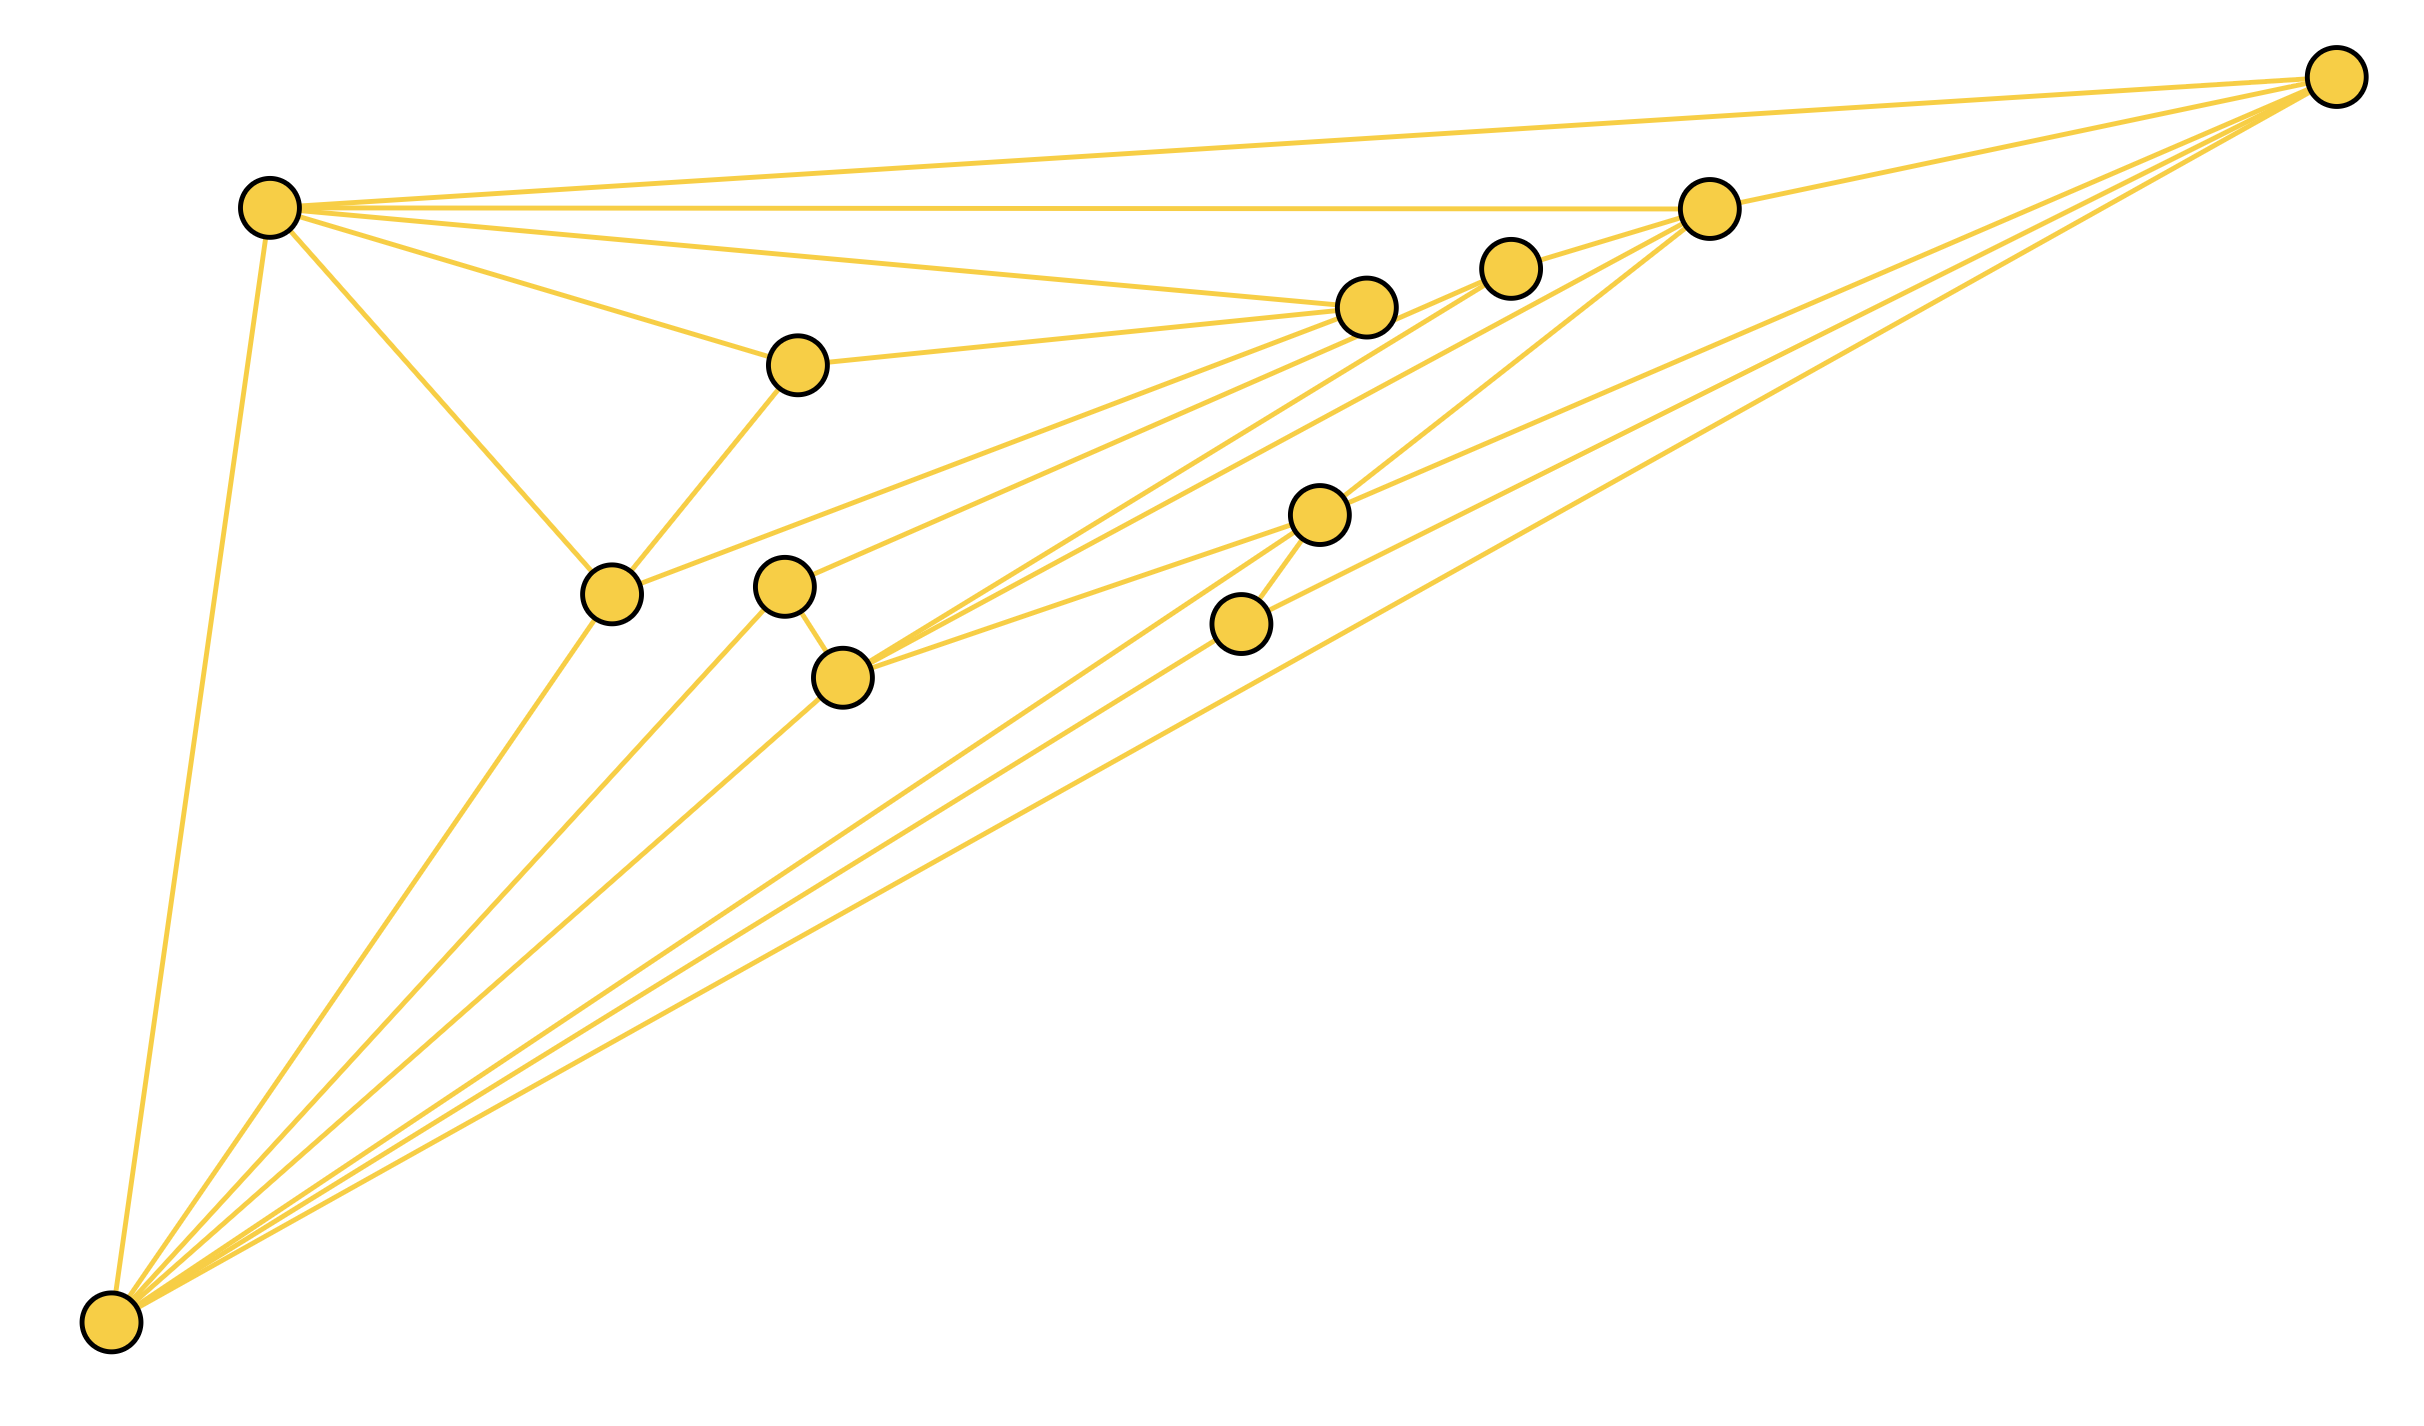
\includegraphics[width=0.4\linewidth]{assets/graph10/12vertices.png}};
                \end{graphfig}
                \qquad
                \begin{graphfig}{}
                    \node at (0,0) {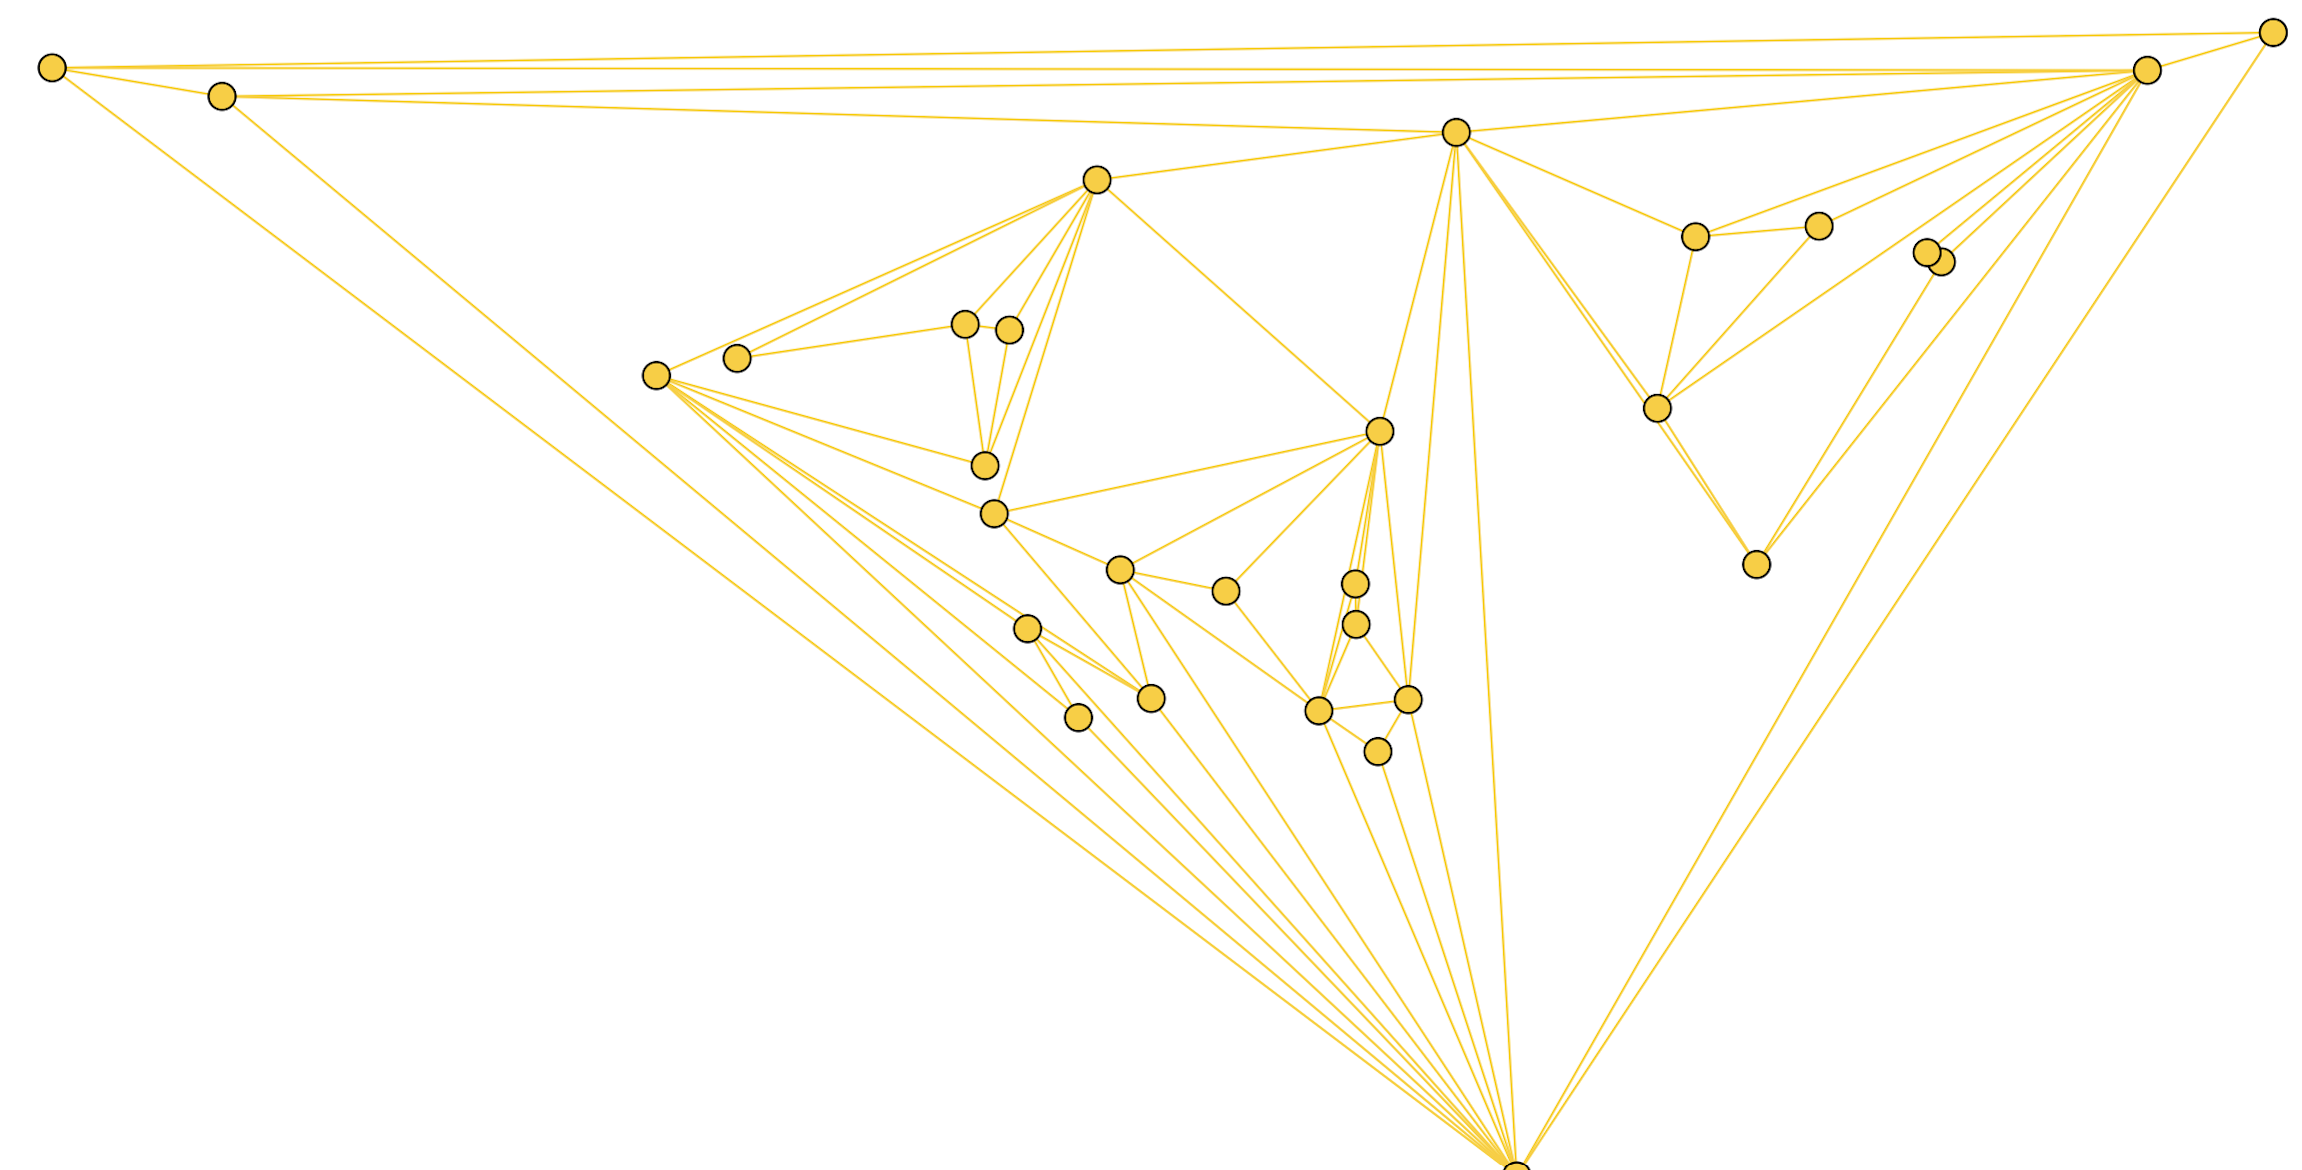
\includegraphics[width=0.4\linewidth]{assets/graph10/30vertices.png}};
                \end{graphfig}
                \begin{graphfig}{NUM}\end{graphfig}
            \end{center}
            The game has been beaten in 12 vertices(left). We have also beaten the game in 30 vertices(right).    
        \end{solution}
        
        \item Draw a tree of order 10. Number the vertices $1-10$. On each edge, write the difference between the numbers. Can you do this so each edge has a different number? Try a different tree. Can you always do it?
        \begin{solution}
        When labeling a tree, using an alternating method guarantees that every edge difference is unique. Instead of picking numbers randomly, you place the labels by swinging back and forth between the smallest and largest remaining numbers. By connecting these alternating pairs along a path, the step by step difference between adjacent vertices automatically creates a clean, descending pattern: The gap between 1 and 10 is 9. The gap between 10 and 2 is 8.This pattern generates every difference from largest to smallest without any duplicates. Even for complex trees with multiple branching arms, applying this strategy—alternating between the smallest and largest available numbers as we move outward from the center—ensures that every single edge ends up with a distinct value.
            \begin{graphfig} {NUM}
                \node[ov] (a1) at (0,2) {1}; 
                \node[ov] (a2) at (-4,0) {2};
                \node[ov] (a3) at (-3,0) {3};
                \node[ov] (a4) at (-2,0) {4}; 
                \node[ov] (a5) at (-1,0) {5};
                \node[ov] (a6) at (0,0) {6};
                \node[ov] (a7) at (1,0) {7};
                \node[ov] (a8) at (2,0) {8};
                \node[ov] (a9) at (3,0) {9};
                \node[ov] (a10) at (4,0) {10};
                \draw (a1)--(a2) (a1)--(a3) (a1)--(a4) (a1)--(a5) (a1)--(a6) (a1)--(a7) (a1)--(a8) (a1)--(a9) (a1)--(a10) {};
            \end{graphfig}
            \begin{graphfig} {NUM}
                \node[ov] (a1) at (0,2) {10};
                \node[ov] (a2) at (-4,0) {9};
                \node[ov] (a3) at (-3,0) {8};
                \node[ov] (a4) at (-2,0) {7};
                \node[ov] (a5) at (-1,0) {6};
                \node[ov] (a6) at (0,0) {5};
                \node[ov] (a7) at (1,0) {4};
                \node[ov] (a8) at (2,0) {3};
                \node[ov] (a9) at (3,0) {2};
                \node[ov] (a10) at (4,0) {1};
                \draw (a1)--(a2) (a1)--(a3) (a1)--(a4) (a1)--(a5) (a1)--(a6) (a1)--(a7) (a1)--(a8) (a1)--(a9) (a1)--(a10) {};
            \end{graphfig} 
            \begin{graphfig} {NUM}
                \node[ov] (a1) at (-5,0) {3};
                \node[ov] (a2) at (-4,0) {5};
                \node[ov] (a3) at (-3,0) {8};
                \node[ov] (a4) at (-2,0) {4};
                \node[ov] (a5) at (-1,0) {10};
                \node[ov] (a6) at (0,0) {1};
                \node[ov] (a7) at (1,0) {9};
                \node[ov] (a8) at (2,0) {2};
                \node[ov] (a9) at (3,0) {7};
                \node[ov] (a10) at (4,0) {6};
                \draw (a1)--(a2)--(a3)--(a4)--(a5)--(a6)--(a7)--(a8)--(a9)--(a10) {};
            \end{graphfig}
        \end{solution}
            \color{blue} RW: This is a very satisfying solution to this problem. I enjoyed reading this! \color{black}
            \color{red}Sorry, I don't wholly believe this. What does this algorithm actually do? How do you pick the next vertex to ``swing" to? And how do you know this works for more complicated graphs? e.g. consider some spanning trees of Petersen.\color{black}
        
        \item \color{red}\textit{CHALLENGE. }\color{black} Is it true that every planar graph has \textit{three} little vertices? Prove or disprove. 
        \item \color{red}\textit{CHALLENGE. }\color{black} \textbf{BY ZANDER}. Prove the \textit{six} color conjecture - that every planar graph can be colored in six colors or less. 
        \begin{enumerate}
            \item Assume not. Then there exists a $G$ s.t. $G$ is plannar and requires more than six colors to color. Let $G$ be a minimal such graph - the one with the smallest order. Then there has to be a little vertex. What can you do if you remove and then put it back? 
        \end{enumerate}
        \item Is $Q_3$ planar? How about $Q_4$? Prove your answers. 
        
        \begin{center}
            \begin{graphfig}{}
                \gqgon{3}{2};
            \end{graphfig}
            \qquad
            \begin{graphfig}{}
                \gqgon{4}{2};
            \end{graphfig}
            \begin{graphfig}{NUM}\end{graphfig}
        \end{center}
        \begin{solution}
            $Q_3$ is planar, $Q_4$ is non-planar. 
        \end{solution}
        \begin{proof} $Q_3$ is drawable like below and is therefore planar. Below is a $K_{3,3}$ inside the alternate drawing of $Q_4$. Since there exists $K_{3,3}$ as a part of the graph, $Q_4$ is non-planar.
            \begin{center}
                \begin{graphfig}{}
                    \node [v] (a1) at (45:3){};
                    \node [v] (a2) at (135:3){};
                    \node [v] (a3) at (225:3){};
                    \node [v] (a4) at (315:3){};

                    \node [v] (a5) at (45:1.5){};
                    \node [v] (a6) at (135:1.5){};
                    \node [v] (a7) at (225:1.5){};
                    \node [v] (a8) at (315:1.5){};
                    \draw (a1)--(a2)--(a3)--(a4)--(a1);
                    \draw (a5)--(a6)--(a7)--(a8)--(a5);
                    \draw (a1)--(a5) (a2)--(a6) (a3)--(a7) (a4)--(a8);
                \end{graphfig}
                \qquad
                \begin{graphfig}{}
                    \gqgon{4}{2};
                    \node [ov] (s1) at (q3){$b1$};
                    \node [ov] (s2) at (q5){$b2$};
                    \node [ov] (s3) at (q15){$b3$};
    
                    \node [ov] (t1) at (q7){$a1$};
                    \node [ov] (t2) at (q11){$a2$};
                    \node [ov] (t3) at (q14){$a3$};
                    \draw [purple, ultra thick] (t1)--(s1);
                    \draw [orange, ultra thick] (t1)--(s2);
                    \draw [green, ultra thick](t1)--(s3);
                    
                    \draw [pink, ultra thick] (t2)--(s1);
                    \draw [violet, ultra thick] (t2)--(q9)--(q13)--(s2);
                    \draw [lime, ultra thick] (t2)--(s3);
                    
                    \draw [magenta, ultra thick] (t3)--(q6)--(q2)--(s1); 
                    \draw [red, ultra thick] (t3)--(q10)--(q8)--(q0)--(q4)--(s2);
                    \draw [teal, ultra thick] (t3)--(s3);
                    
                \end{graphfig}
                \begin{graphfig}{NUM}\end{graphfig}
                %                  sorry zander. 
            \end{center}
            The following glossary may aid you in navigating $Q_4$ :
            $$
            \begin{vmatrix}
                \color{purple} a1-b1 & \color{orange} a1-b2 & \color{green} a1-b3 \\
                \color{pink} a2-b1 & \color{violet} a2-b2 & \color{lime} a2-b3 \\
                 \color{magenta} a3-b1 & \color{red} a3-b2 & \color{teal} a3-b3 
            \end{vmatrix}
            $$\color{black}. 
        \end{proof}
                \color{blue} RW: Well this took some time! LOl, very good work. The only thing I would have done to REALLY solidify your response was explain the significance of the coloring to show the planarity (or lack thereof). Why is it that the coloring of your image makes $Q_3$ planar? \color{black}
                \color{red}$Q_3$ is the one on the left. The one drawn in the plane with no crossings. But yeah, good work finding a $K_{3,3}$ subdivision in $Q_4!$\color{black}
    
        \item Find a socially optimal way to seat these people, and justify why your answer is correct. You will have to come up with a good definition of "socially optimal". 
        \begin{graphfig}{NUM}
            \node at (0,0) {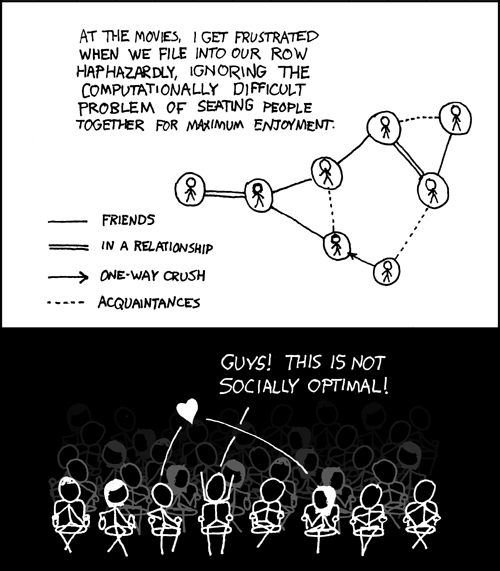
\includegraphics[width=0.5\linewidth]{assets/ohno.png}};
        \end{graphfig}
        \begin{solution}
            To interpret the given graph, we can say A and B, F and G are in a relationship. B\&C, B\&E, E\&F, G\&H are friends, and D has a crush on C. To seat people in a "socially optimal way, we first prioritize couples. We want couples to sit together (couples being those who are in a relationship). Then, the next priority would be friends followed by those with one way crushes. Based on that criteria we can make the seating arrangement as follows.
            
            \begin{graphfig} {NUM}
                \node[ov] (a1) at (-5,0) {D};
                \node[ov] (a2) at (-4,0) {C};
                \node[ov] (a3) at (-3,0) {A};
                \node[ov] (a4) at (-2,0) {B};
                \node[ov] (a5) at (-1,0) {E};
                \node[ov] (a6) at (0,0) {F};
                \node[ov] (a7) at (1,0) {G};
                \node[ov] (a8) at (2,0) {H};
                \draw (a1)--(a2)--(a3)--(a4)--(a5)--(a6)--(a7)--(a8);
            \end{graphfig}
        \end{solution}

        \color{blue} RW: I made a couple of tweaks to the wording of your response for this problem to clear up some grammatical mistakes and to make your answer more comprehensive. If I mis-interpreted what you said, my sincere apologies. Feel free to change it back if you need :) \color{black}
        \\
        \item \color{green}\textit{OPEN ENDED. }\color{black} What conjectures / theorems can you com up with about Graph Reconstruction? This is what research math can be like. Explore and \color{red} ARGUE\color{black}.
        \item  \color{blue}\textit{UNSOLVED. }\color{black} \textit{Kotzig-Ringel Graceful Tree Conjecture}. For every tree of order $n$ you can number the vertices $1,2,\dots n$ such that $n-1$ distinct differences appear on the edges. In other words, for every edge you take the difference between the numbers you gave the vertices. You can always number the edges such that all those differences are distinct. Can you prove that the K-R GTC is always true? Can you find a counterexample? 


        \color{blue} Really quality work here team! I hope that you enjoyed today and I cannot wait to see your final homework assignment tomorrow evening!\color{black}
    \end{enumerate}
\end{document}